\chapter{Lecture 2: Connectedness}
\section{Connected Sets}
\begin{definition}
    [Connected Set]
    An \textit{open} set $D$ is connected if each pair of points $p, q \in D$ can be joined by a polygonal path lying entirely in $D$. That is:
    \[
        \exists P_2, P_3, \ldots, P_n \in D\quad  \text{ such that }\quad  pP_1, P_1P_2, \ldots, P_nq \in D\]
\end{definition}

\begin{remark}
    The set doesn't \textit{have} to be open, but it is easier to prove connectedness for open sets.
\end{remark}

\begin{figure}[H]
    \centering
    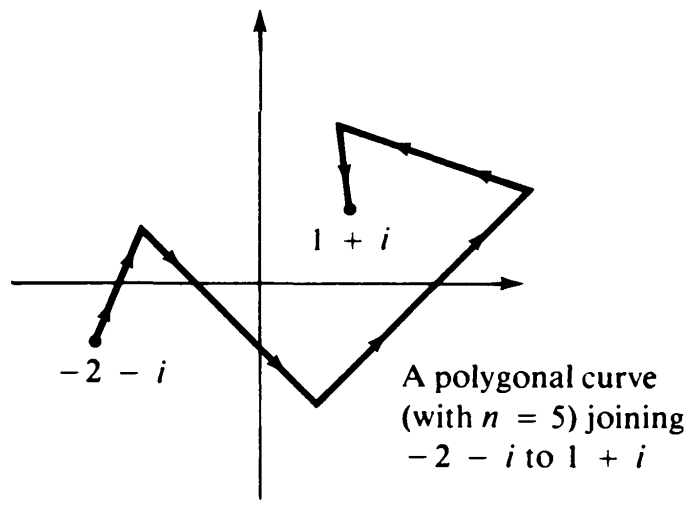
\includegraphics[scale=0.5]{LECTURE_2/poly.png}
    \caption{Polygonal Path}
    \label{fig:poly}
\end{figure}

\begin{definition}
    [Domain]
    A domain is a set that's
    \begin{itemize}
        \item Open
        \item Connected
        \item Not empty
    \end{itemize}
\end{definition}

\begin{definition}
    [Convex Set]
    A set $D$ is convex if for each pair of points $p, q \in D$, the line segment $pq$ lies entirely in $D$.
\end{definition}

\begin{figure}[H]
    \centering
    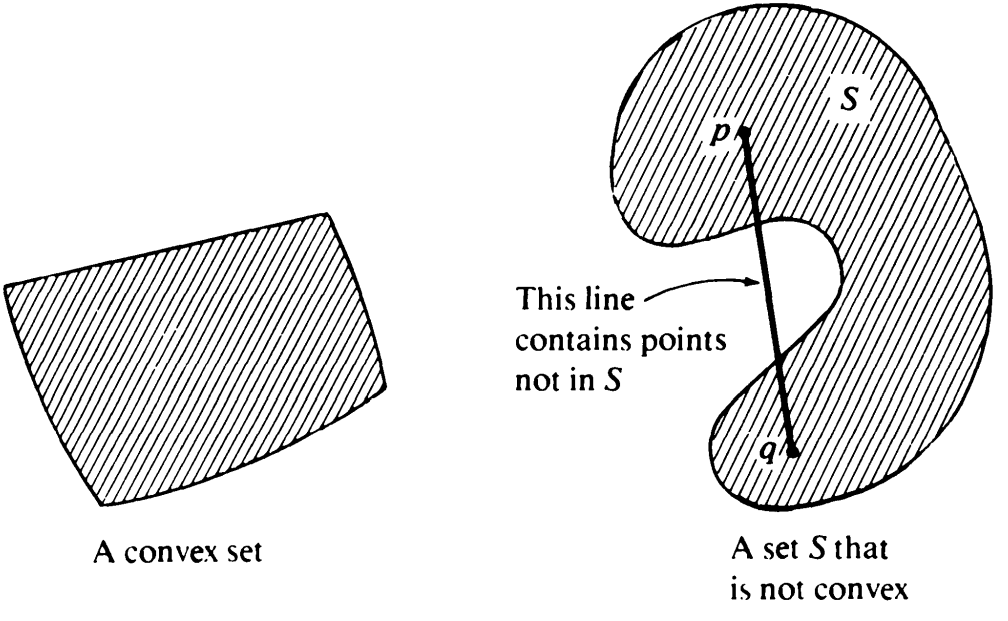
\includegraphics[scale=0.5]{LECTURE_2/convex.png}
    \caption{Convex Set}
    \label{fig:convex}
\end{figure}

\begin{theorem}
    [Convex $\implies$ Connected]
    If $D$ is a convex open set, then $D$ is connected.
\end{theorem}

\begin{definition}
    [Open Half-plane]
    A set $D$ is an open half-plane if it is of the form
    \[
        D = \{z \in \mathbb{C} : \Re\{az + b\} > 0\}
    \]
    \textit{Each open half-plane is convex and open}
\end{definition}

\begin{definition}
    [Closed Half-plane]
    A set $D$ is a closed half-plane if it is of the form
    \[
        D = \{z \in \mathbb{C} : \Re\{az + b\} \geq 0\}
    \]
    \textit{Each closed half-plane is convex and closed}
\end{definition}

\section{Point at Infinity}
\begin{definition}
    [Point at Infinity]
    A set is said to contain the point at infinity if it contains all points $z$ such that $|z| > R$ for some $R > 0$.
\end{definition}

\begin{example}
    No open Half-plane contains the point at infinity. Even though the set is unbounded, choosing $R$ near the boundary will always give a point outside the set.
\end{example}

\section{Functions and Limits}

\begin{definition}
    [Limit of a Sequence of Complex Numbers]
    \begin{align}
         & \lim_{n \to \infty} z_n = z \quad \text{or}\quad z_n \to z \iff \forall \epsilon > 0, \exists N \in \mathbb{N} \\
         & \text{such that} \quad n \geq N \implies |z_n - z| < \epsilon
    \end{align}
\end{definition}

\begin{corollary}
    [Parts of a Limit]
    If $z_n = x_n + iy_n$ and $z = x + iy$, then
    \[
        \lim_{n \to \infty} z_n = z \iff \lim_{n \to \infty} x_n = x \text{ and } \lim_{n \to \infty} y_n = y
    \]
\end{corollary}

\begin{theorem}
    [Subsequence]
    Suppose $\{z_n\}$ converges with limit $z$. Then every subsequence, $z_{m_n} = f(n)$ also converges to $z$. Where $ 1 \leq m_1 < m_2 < \ldots$
\end{theorem}

\begin{definition}
    [Limits of Functions]
    \begin{align}
         & \lim_{z \to z_0} f(z) = w \iff \forall \epsilon > 0, \exists \delta > 0     \\
         & \text{such that}\quad 0 < |z - z_0| < \delta \implies |f(z) - w| < \epsilon
    \end{align}
\end{definition}

\section{Continuity}
\begin{definition}
    [Continuous Function]
    A function $f(z)$ is continuous at $z_0$ if
    \[
        \lim_{z \to z_0} f(z) = f(z_0)
    \]
\end{definition}

\begin{corollary}
    [Continuous at Infinity]
    A function $f(z)$ can be continuous at $\infty$ if $f(\infty) = \lim_{z\to \infty}f(z) = f(\infty)$. Note, $f(\infty)$ may equal $\infty$ \\
    \textit{This is equivalent to saying that $f(1/z)$ is continuous at $z = 0$}
\end{corollary}